\begin{center}
\begin{tikzpicture}
	\node[anchor=south west,inner sep=0] (image) at (0,0) {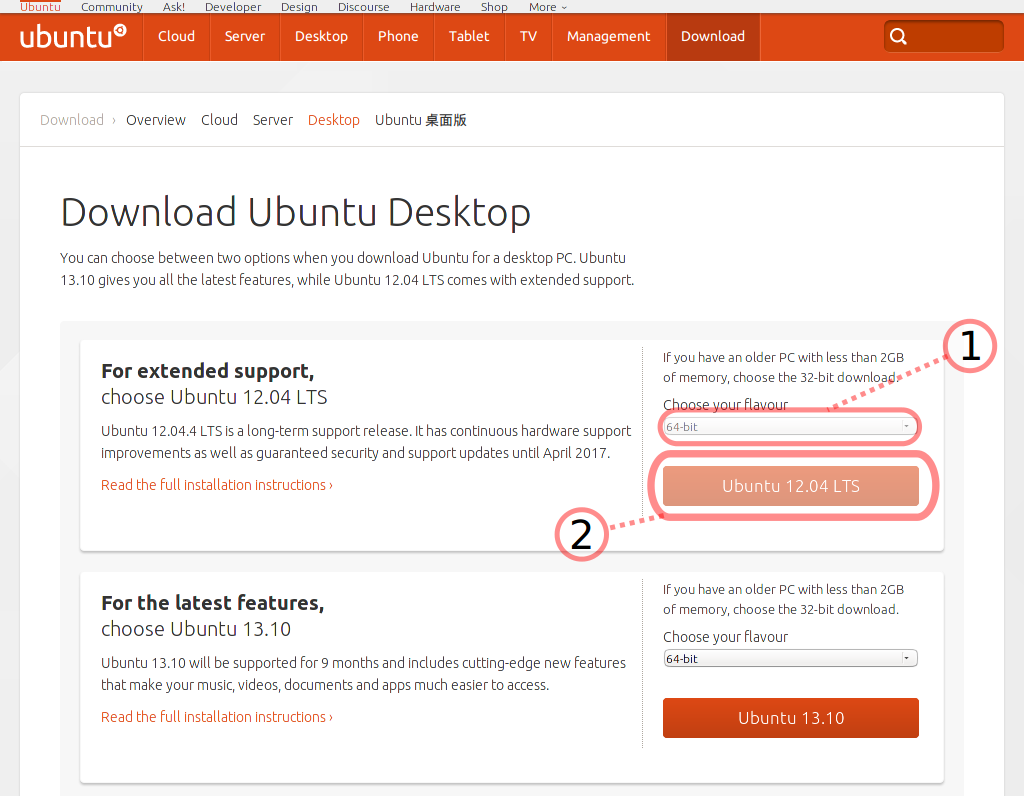
\includegraphics[width=\linewidth]{images/instalacja_pobieranie_obrazu.png}};
	\begin{scope}[x={(image.south east)},y={(image.north west)}]
		\draw[ubuntu_orange,line width=3pt,rounded corners] (0.66,0.38) rectangle (0.95,0.49);
		\draw[ubuntu_orange,line width=3pt,fill=white,fill opacity=0.75] (0.55,0.55) circle [radius=0.5cm]
			node[text=black]{\Huge \textbf 1};
		\draw[ubuntu_orange,dashed,line width=3pt] (0.58,0.55) -- (0.66,0.45);		
		
		\draw[ubuntu_orange,line width=3pt,rounded corners] (0.66,0.22) rectangle (0.95,0.36);
		\draw[ubuntu_orange,line width=3pt,fill=white,fill opacity=0.75] (0.55,0.15) circle [radius=0.5cm]
			node[text=black]{\Huge \textbf 2};
		\draw[ubuntu_orange,dashed,line width=3pt] (0.58,0.15) -- (0.66,0.28);
		
    \end{scope}
\end{tikzpicture}
\end{center}

Pierwszym etapem instalacji systemu jest pobranie instalatora. W tym celu otwórz stronę\linebreak[4] \href{http://www.ubuntu.com/download/desktop}{ubuntu.com} i z górnego paska wybierz \textcolor{ubuntu_orange}{Download}, a następnie \textcolor{ubuntu_orange}{Desktop}.

\begin{enumerate}[label=\protect\circled{\arabic*}]
\item To pole pozwoli ci wybrać pomiędzy 32- lub 64-bitową wersją systemu. Domyślnie wybrana jest wersja 64-bitowa.
\item Kliknij ten przycisk, aby przejść dalej.
\end{enumerate}

Następnie będziesz mieć możliwość przekazania dotacji na rzecz Ubuntu. Nie będziemy się tym teraz zajmować. Przewiń stronę w dół i kliknij \textcolor{ubuntu_orange}{Not now, take me to the download}. Zostaniesz przeniesiony na kolejną stronę, a po kilku sekundach rozpocznie się pobieranie obrazu systemu.

Jeżeli twój komputer został wyprodukowany nie dawnej niż 5 lat temu, wersja 64-bitowa będzie na pewno odpowiednia. Jeżeli masz mniej niż 2 gigabajty RAM-u, wybierz wariant 32-bitowy. Niezależnie od tego, jaką wersję wybierzesz, i tak będziesz mieć dostęp do takiego samego zestawu oprogramowania. Wariant 64-bitowy jest lepiej dopasowany do nowoczesnych komputerów, jeżeli jednak masz jakiekolwiek wątpliwości, wybierz wersję 32-bitową. Będzie ona działać także na 64-bitowym komputerze, choć nie będzie wykorzystywać wszystkich jego możliwości. Jeżeli twoja płyta główna kontrolowana jest przez UEFI, musisz wybrać system 64-bitowy.

Linki do pobierania bezpośredniego:
\begin{itemize}
\item \href{http://releases.ubuntu.com/14.04/ubuntu-14.04-desktop-amd64.iso}{wersja 64-bitowa (964 megabajty);}
\item \href{http://releases.ubuntu.com/14.04/ubuntu-14.04-desktop-i386.iso}{wersja 32-bitowa (970 megabajtów);}
\item \href{http://releases.ubuntu.com/14.04/ubuntu-14.04-desktop-amd64+mac.iso}{wersja 64-bitowa dla komputerów MAC (962  megabajty).}
\end{itemize}
